Using a team of robots to explore and build the map of an unknown environment is the basic task of many multi-robot applications.
This work target 2D multi-robot exploration, because current practical applications, such as self-driving cars, home service robots, and multi-robot rescue, are mainly based on 2D AGV platforms.

In terms of perception of multi-robot exploration, the robots in this team need to do Distributed Simultaneous Localization and Mapping (DSLAM) to share their understanding of the environment, build a global map together, and provide the location of each robot in this map.
In terms of decision, the robots need to direct themself to explore unknown space, thus expanding the known and explored area of a map which is updated while doing the DSLAM.

It is a common practice to use external positioning signals (e.g. GPS, motion capture) to provide the location of the robots. 
Yet in communication constrained environments, such as cave exploration and building inspection, the external positioning signals will be shielded. 
Some previous works implement DSLAM systems \cite{cieslewski2018data,lajoie2020door, schmuck2019ccm} to provide the location in these nonideal environments. 
The basic idea of these DSLAM is similar: 1) adopting single-robot SLAM system to provide intra-robot location, 2) sharing \& matching place recognition infomation to detect the inter-robot loop closures, 3) transmitting the sensor data related to the recognized same place to calculate relative poses (RelPose) and 4) merging \& optimizing the single-robot SLAM results according to the relative poses. 
These systems use camera image to extract a sophisticated feature vector to encode the place information. 
% Computing the distance between feature vectors can know if robots experience the same place. 
These feature vectors can be generated form the handcrafted method \cite{jegou2014triang} or emerging neural-network-based method \cite{radenovic2018fine, arandjelovic2016netvlad}. 
However, these image-based  method is communication-costing to share the feature vectors. 
Besides sharing place information, the corresponding sensor data (camera images or laser scans), which are also communication-costing, need to be transmitted between robots to get the relative pose (RelPose).
DSLAM systems are also vulnerable to mistaken place recognition. Some works develop outlier rejection method using temporal information \cite{cieslewski2018data} and geometric verification \cite{lajoie2020door}. 
However, these outlier rejection methods needs the robot trajectories overlap with others in an area to provide extra temporal or geometric constrains.

Frontier-based exploration strategies are usually used in robotic exploration for both single-robot and multi-robot exploration \cite{senarathne2013efficient, umari2017autonomous, orvsulic2019efficient}.
The flow of these frontier-based methods are: 1) detecting points on the frontier edges of the map, which separate the explored space and the unknown space, and 2) assigning one of the frontier point to the robot as its goal for exploration. 
Because only one goal point needs to be sent to the robot, frontier based methods are can be easily deployed on the real robot with the help of ROS framework \cite{quigley2009ros}.
However, previous works mainly focus on shortening the exploration time and exploring path length. 
When use these methods together with DSLAM systems for multi-robot exploration, the trajectories of different robots may not sufficiently overlap, resulting in the failure of place recognition.

\begin{figure*}[t]
    \centering
    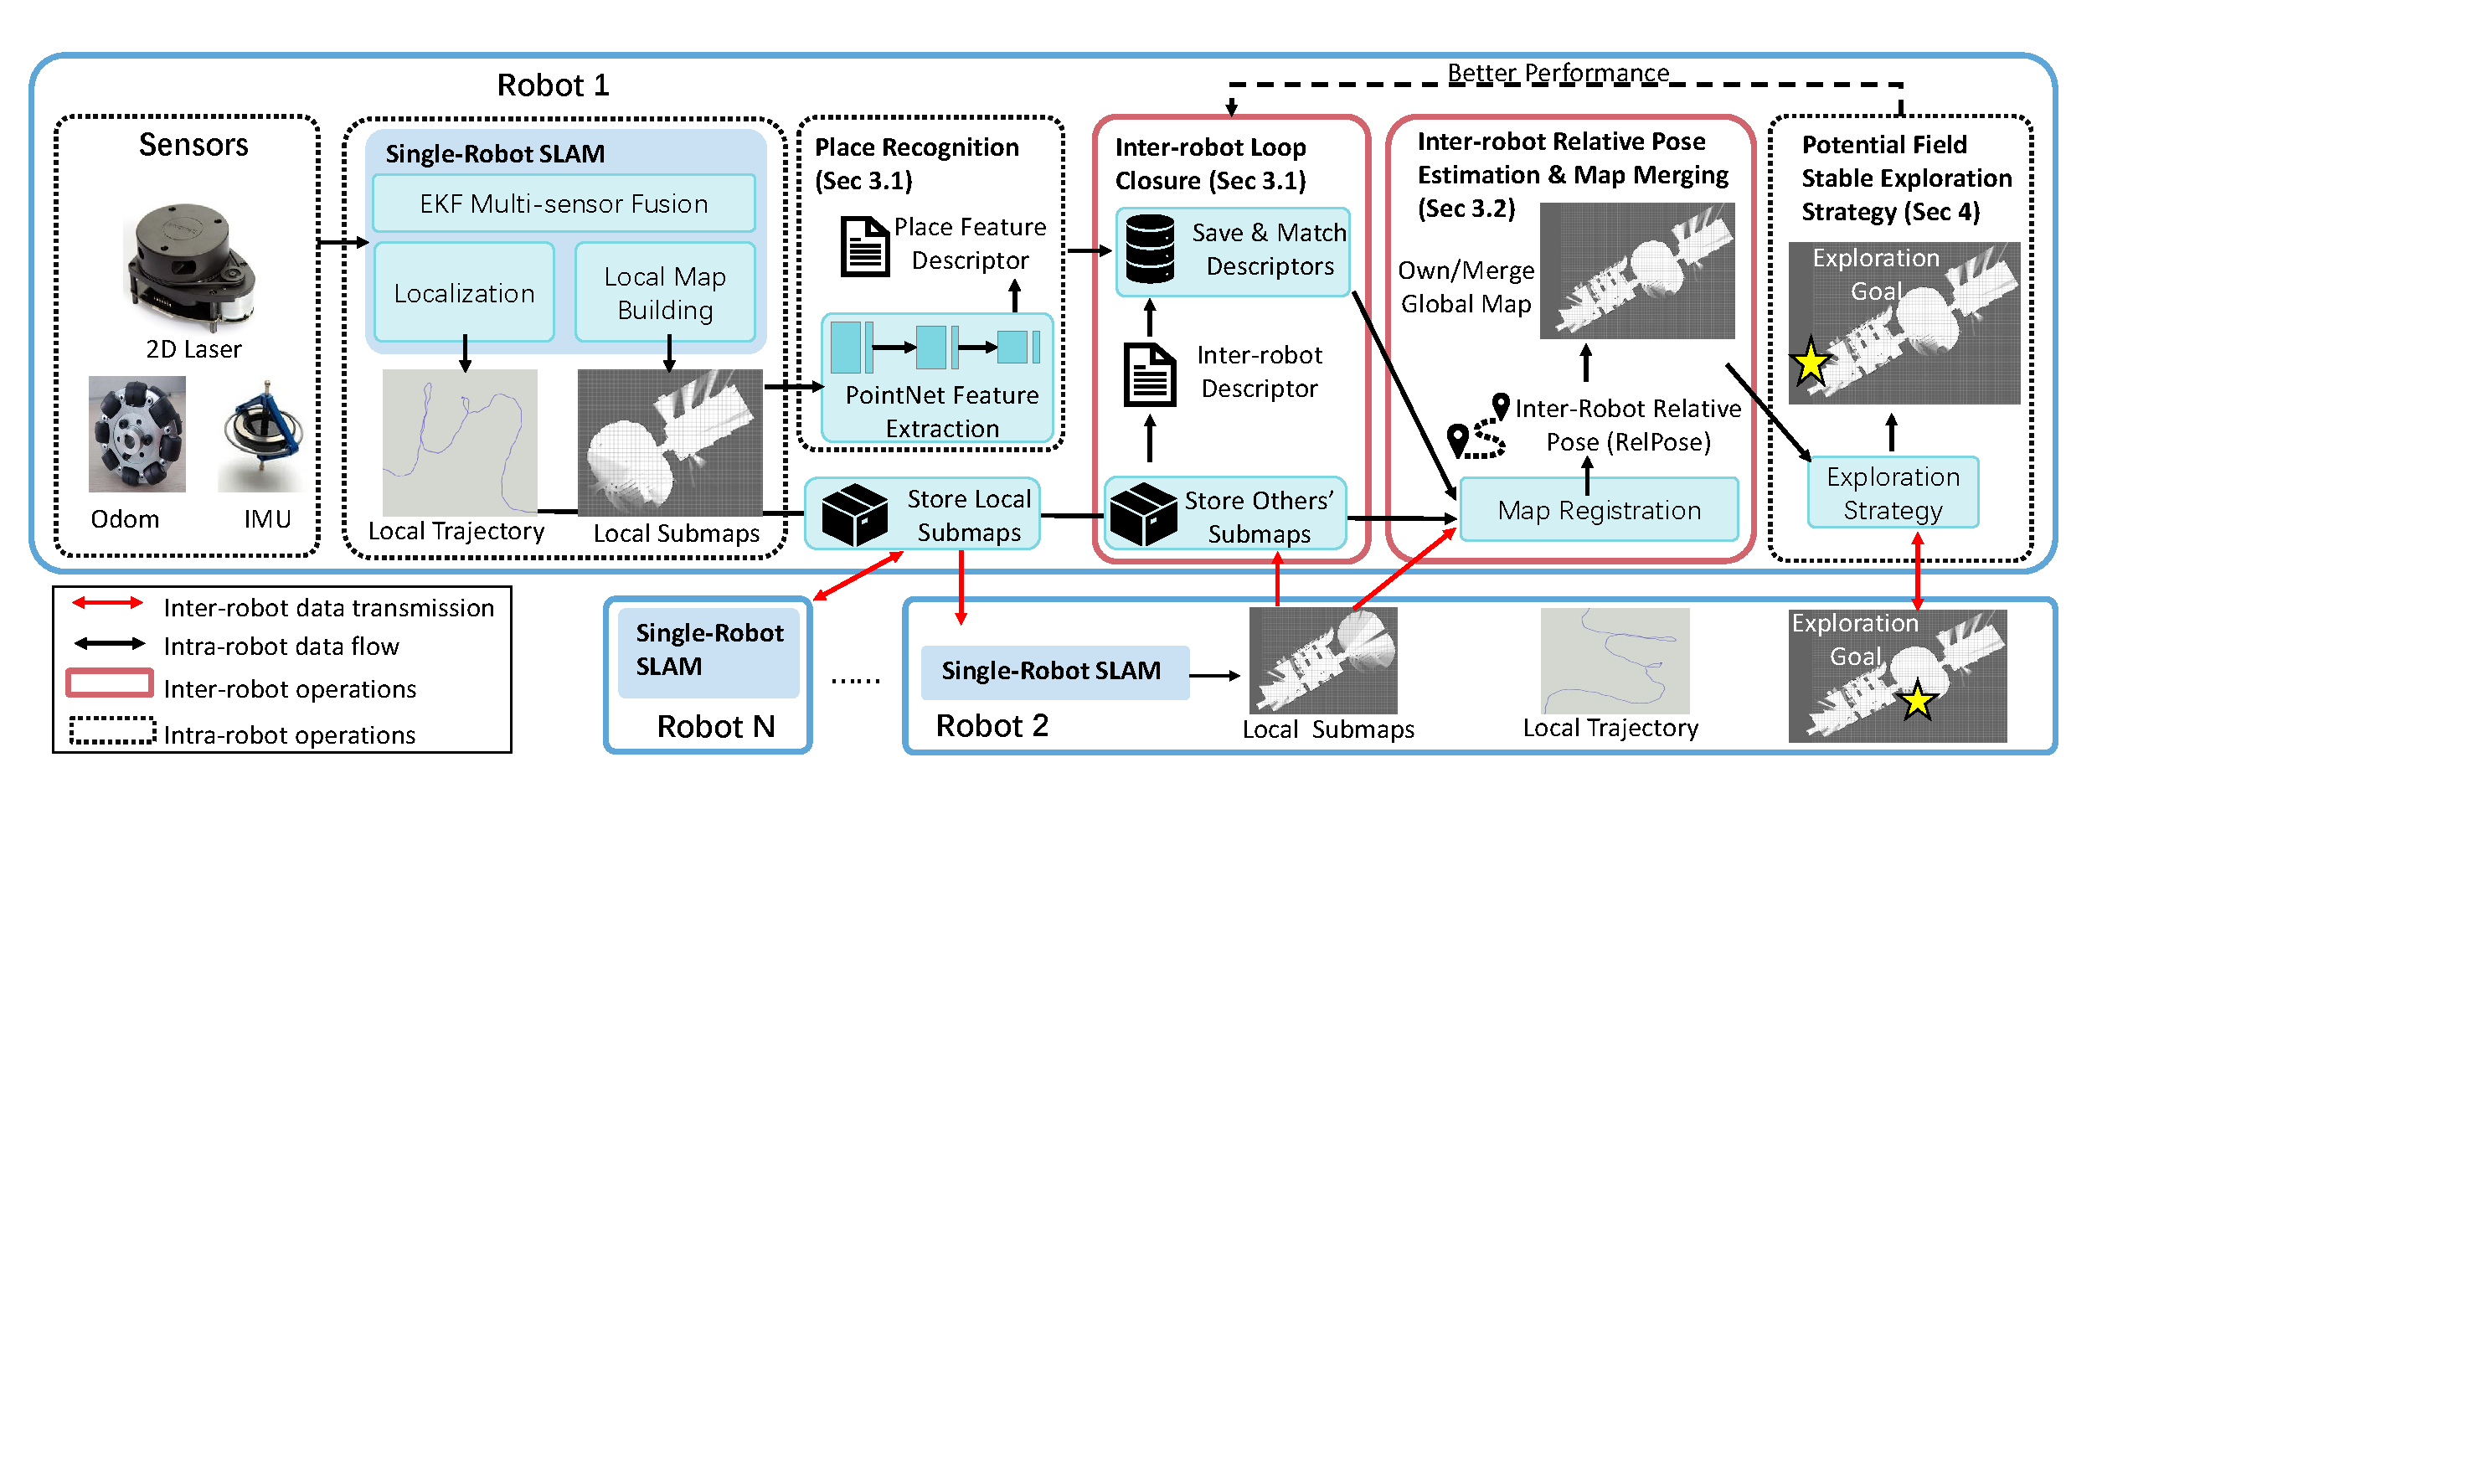
\includegraphics[width=0.99\linewidth]{fig/dataflow.pdf}
    \caption{The system overview of our multi-robot exploration system. All the infomation transmitted between robots are the submaps (the local maps \& the location of each local map on the trajectory). 
    The place descriptor is generated for each self and other's submap. The descriptor is recorded and used for place matching. 
    As the same place are detected between different robots, the relative pose (RelPose) of these robots are also calculated from the shared submaps, and the submaps are merged into a global map. 
    Finally, the stable exploration method will assign each robot to different unknown spaces if they konw the position of each other. 
    Otherwise, the stable exploration method will guide the robots to the explore through a stable path so that they may meet a same place. }
    \label{fig:sysframe}
\end{figure*}

To address the aforementioned problems about communication traffic and place recognition efficiency. We propose a data-efficient multi-robot  exploration system with the following contributions:

\begin{itemize}
    \item We use local occupancy grid submaps instead of camera images to extract feature vectors for place recognition. We use neural-network (NN) to provide rich feature for 
    \item We also use the submaps instead of the sensor data (laser scan) to estimate the relative pose (RelPose) between robots.
    \item We introduce the idea of potential field to frontier-based exploration strategy to generate stable exploration paths to provide overlapped trajectories for better place recognition performance.
\end{itemize}



As illustrated in \Cref{fig:sysframe}. the single-robot SLAM method (we use Cartographer \cite{hess2016real} in this work) builds the submaps, which include the local map of an area within a region and its location on the exploration trajectory, according to the lidar scan, wheel odometery and IMU sensors.
Each submap is shared between robots, a CNN-based method extracts each submap into a feature vector for further matching to detect inter-robot loop closures.
The submap is also used to estimate the relative pose between robots according to the inter-robot loop closures.
Before detecting the inter-robot loop closures, the robot merge the single-robot local submaps to produce its own global map. 
The stable exploration method will guide the robot on its own global map through a stable path to meet a same place with others while exploring the unknown area.
After detecting the inter-robot loop closures, the robots will merge its own submap and orthers' to build a merged global map. The different robots will be assigned to different unknown area for better exploration efficiency.


The rest of this article is organized as follows: \Cref{sec:relatedwork} introduces the related works. The submap-based DSLAM system is shown in \Cref{sec:dslam}. The stable exploration path generation method is detailed in \Cref{sec:exploration}. The results and evaluation are listed in \Cref{sec:experiment}. \Cref{sec:conclusion} will conclude this paper.